\section{Robust and Noise Resilient Training}

\begin{frame}{Easily Saturated Photonic Activation Functions}
  % The unique nature of optical non-linearities:
  \begin{center}
       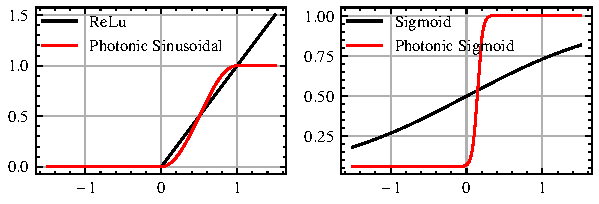
\includegraphics[width=0.9\textwidth]{./sections/1_adaptinit/imgs/activations.pdf}
  \end{center} \vspace{-10pt}
  \begin{itemize}
  \item \textcolor{red}{Facing challenges to support traditionally used activation functions such as ReLu}
  \item \textcolor{red}{Mostly relying on high slope functions such as
      sinusoidal- or sigmoidal-based}
  \end{itemize}
\end{frame}


\begin{frame}{Vanishing Gradients}
\begin{center}
    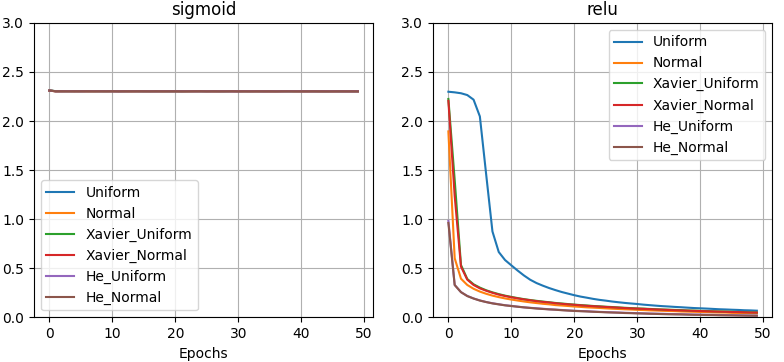
\includegraphics[width=0.9\textwidth]{./sections/1_adaptinit/imgs/specific_initialization.png}
\end{center}
    \begin{itemize}
        \item \textbf{Susceptible to vanishing gradient phenomena}
        \item \textbf{Making PNNs especially sensitive to the initialization scheme} 
    \end{itemize}
\end{frame}


\begin{frame}{Typically Weights Initialization}

  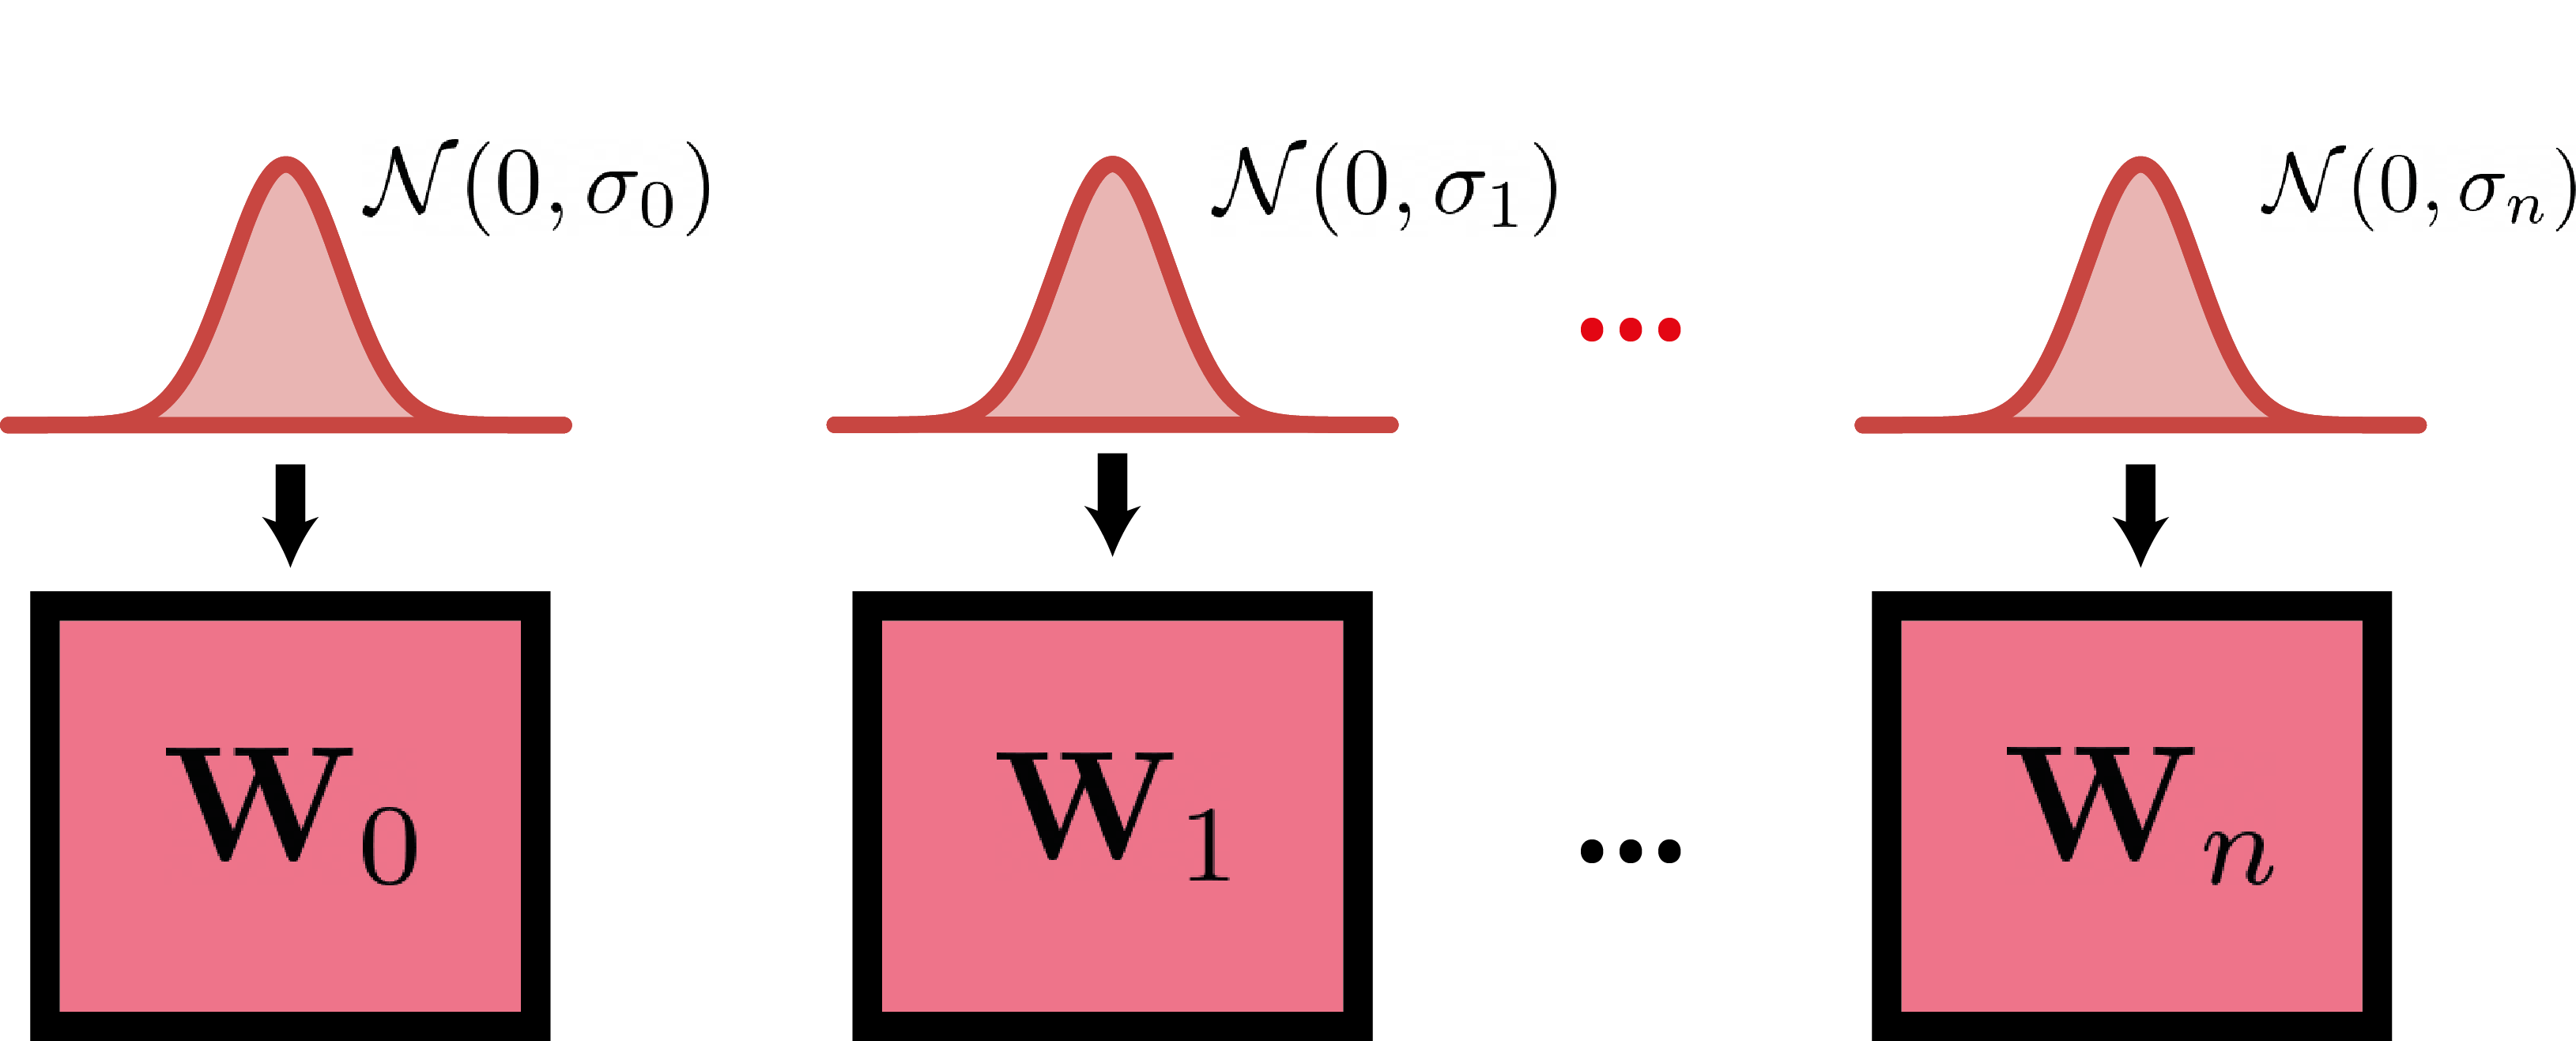
\includegraphics[width=\linewidth]{sections/1_adaptinit/imgs/adapt_init_1.png} \vspace{10pt}
  
    Typically the \textbf{weights of \(i\)-th layer are initialized by
    drawing from a Gaussian distribution} with zero mean and \(\sigma^2_i
  \in \mathbb{R}\) variance, denoted by $\mathbf{W}_i \sim
  \mathcal{N}_{N_{i} \times N_{i-1}}(0,
  \sigma^2_i)$. 
\end{frame}

\begin{frame}{Limitation of Initialization methods} % Here I can also add Xavier and He initialization
    \textbf{Vanishing gradient phenomena have been extensively studied for regular training}.
    \begin{itemize}
        \item \textcolor{red}{Such schemes target traditionally used activation functions}
        \item \textcolor{red}{Consider only the size of every layer (fan-in and fan-out)}
        \item \textcolor{red}{Ignoring the synergistic effects during inference (such as noise)}
    \end{itemize}
    \textcolor{red}{\textbf{Leading to suboptimal results and limiting the performance of models in such systems.}}
  \end{frame}


\begin{frame}{Thesis Contribution}
  An unified \textbf{hardware-aware training framework} that incorporates: 
  \begin{itemize}
    \item \textbf{Photonic transfer functions} in the optical configuration
    \item Easily saturated \textbf{photonic activation functions}
    \item Inevitable \textbf{noise sources} exists during hardware inference
    \end{itemize}
    
    % The proposed method is an \textbf{architecture-agnostic} method that
    % deals with both \textbf{initialization of trainable parameters} and actual \textbf{weight
    % update} in gradient-based optimization.

    % Establishing a more holistic co-design approach in training process. 
\end{frame}


% \begin{frame}{Establishing Objective}
% 	The information flow through network can be theoretically modeled by the
%   Markov chain rule: 
%   \begin{equation}
%     Y \rightarrow X \rightarrow \hat{X}_1  \rightarrow \dots \rightarrow \hat{X}_M \rightarrow \hat{Y},
%   \end{equation}
%   {\scriptsize   where \(X\) be the input random variable (input to the ANN), Y the target variable,
%   and \(\hat{Y}\) the final network prediction as acquired through a series of
%   layer transformations \(\hat{X}_1, \dots \hat{X}_M\). } \vspace{15pt}

%     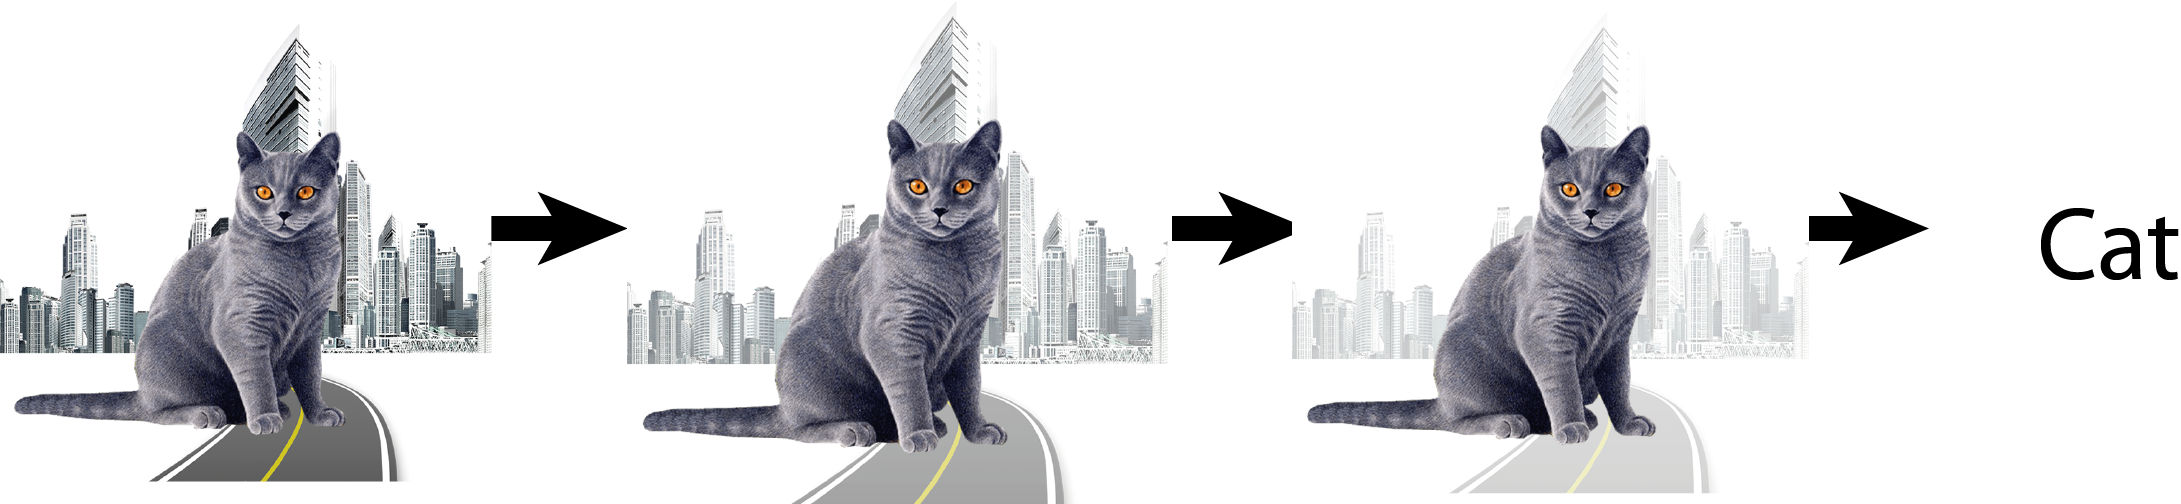
\includegraphics[width=0.9\linewidth]{sections/1_adaptinit/imgs/info_0.png}

% \end{frame}


% \begin{frame}{Suboptimal Initialization}

%   The information lost in one layer cannot be recovered later in subsequent
%   layers.
%   \begin{equation}
%     I(Y; X) \geq I(Y; \hat{X}_1) \geq \dots \geq I(Y; \hat{X}_M) \geq I(Y;\hat{Y}).
%   \end{equation} \vspace{15pt}

%   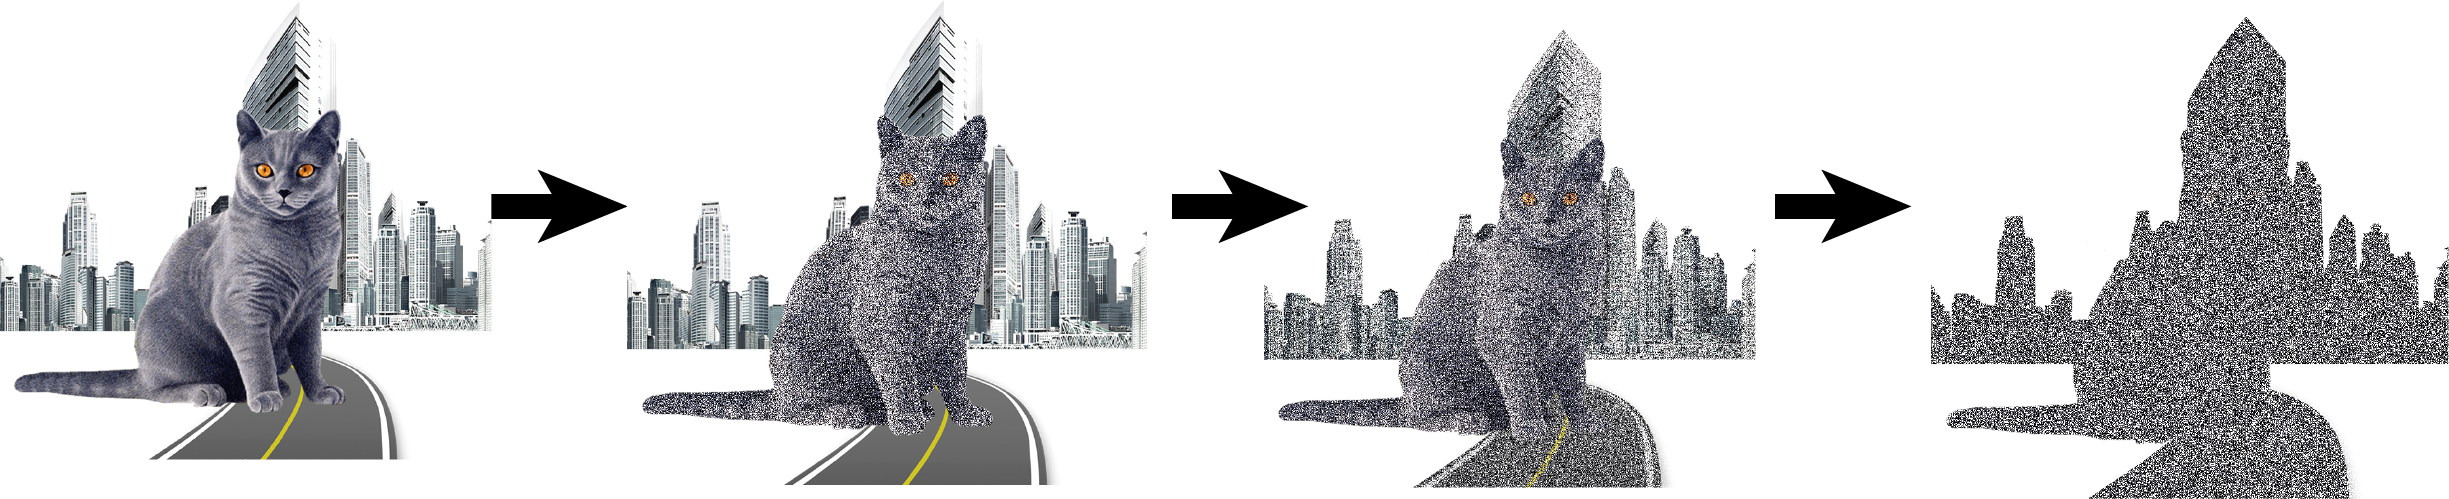
\includegraphics[width=\linewidth]{sections/1_adaptinit/imgs/info_1.png}

% 	% Now suppose that due to a suboptimal initialization scheme, we have suppressed
%   % most information about \(Y\) in the first layer, i.e., \(I(Y; \hat{X}_1) =
%   % \epsilon\). Then this implies that:
%   % \begin{equation}
%   %   I(Y; \hat{Y}) \leq I(Y; \hat{X}_M) \leq  \dots \leq I(Y; \hat{X}_2) = \epsilon.
%   % \end{equation}
%   % Therefore, we cannot retrieve any
%   % additional information about \(Y\) after this layer.
% \end{frame}

% \begin{frame}{Initialization Objective}
% 	% Also, note that ``compressing'' in such a way that irrelevant information
%   % about \(Y\) is beneficial, since it allows us to acquire representations that
%   % discard irrelevant information and keep only the factors that explain \(Y\).
%   % Deep Learning process can be seen as a process of finding approximate minimal
%   % sufficient statistics about \(Y\),  
%   % \[\mathcal{L} = I(X; \hat{Y}) - \alpha I(Y; \hat{Y}),\] where \(\alpha\)
%   % controls the trade-off between the compression rate and the information
%   % preserved about \(Y\).

%     The initialization can be formulated as an optimization problem that targets
%     maximize the information for the \(k\)-th layer: 
%     \begin{equation}
%      \begin{aligned}
%          \text{maximize } \quad &  I(Y_k, \hat{Y}), \text{ }  \forall k \in [0, M],\\
%          \text{s.t. } \quad &  \bm{W}_{k} \sim N(0,a_k\sigma^2), \\
%          & a_k > 0, \\
%     \end{aligned}
%   \end{equation}
%   {\scriptsize where \(M \in \mathbb{N}\) is the number of layers.} \vspace{15pt}

%  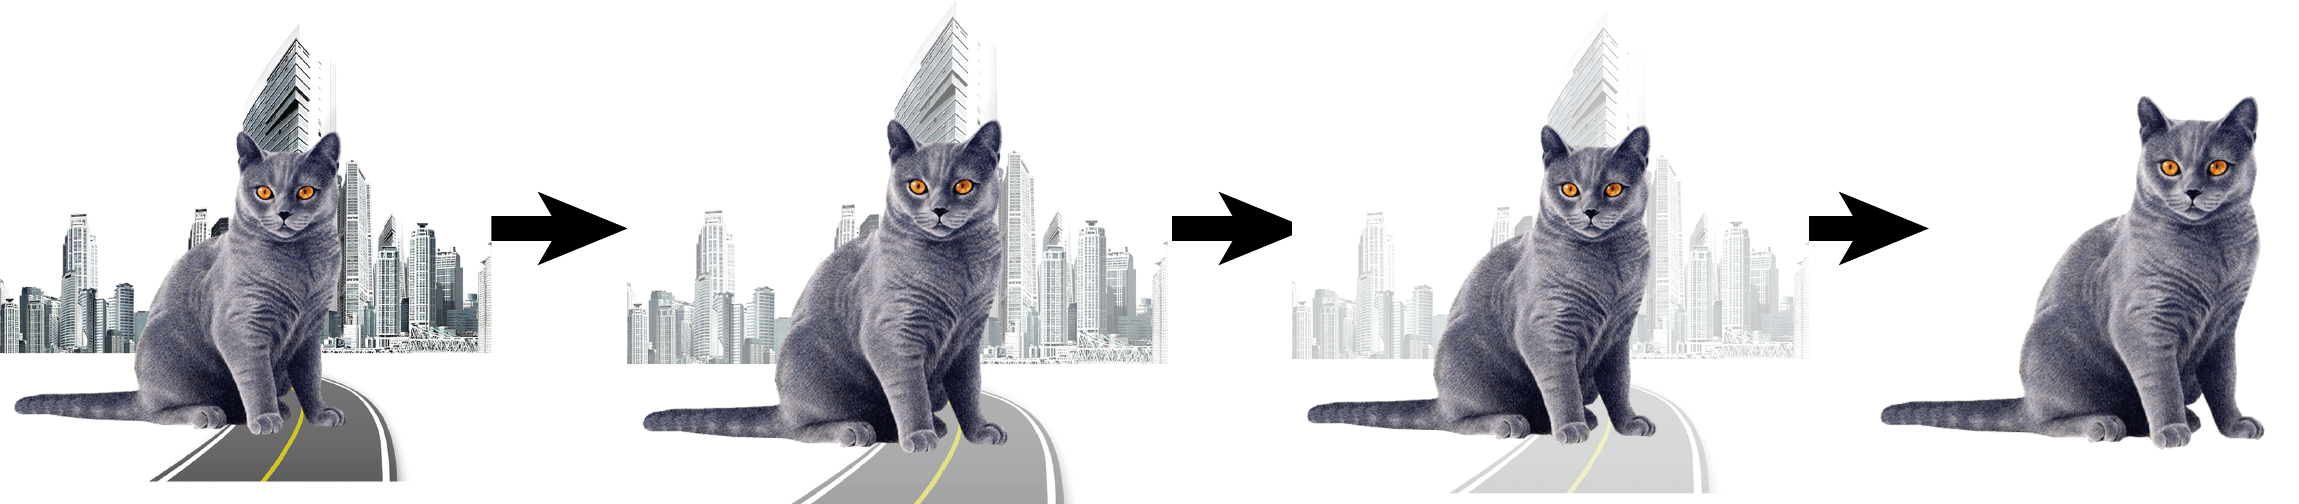
\includegraphics[width=\linewidth]{sections/1_adaptinit/imgs/info_2.png}
% \end{frame}



\begin{frame}{Tranable Scaling Factor}
	  An additional \textbf{scaling factor} \( \{a_{i} \in \mathbb{R} \text{ , }
  i = [0, \ldots, M]\}\) is introduced for each layer: 
  \begin{equation}
    \bm{y}_{i} = f_{i}(a_i, \bm{W}_i, \bm{b}_i;\bm{y}_{i-1}) =  g_{i}{(|a_{i}|\bm{W}_{i}\bm{y}_{i-1} + \bm{b}_i)} \in \mathbb{R}^{N_i},
  \end{equation}
  {\scriptsize where \(|\cdot|\) denotes the absolute value operator,
    \(g_{i}(\cdot): \mathbb{R}^{N_{i-1}} \rightarrow \mathbb{R}^{N_{i-1}}\), the
    activation functions, \(\bm{W}_i \in \mathbb{R}^{N_{i} \times N_{i-1}}\) and
    \(\bm{b}_i \in \mathbb{R}^{N_{i}}\) are the weights and biases of the layer,
    respectively.} 

    \begin{center}
        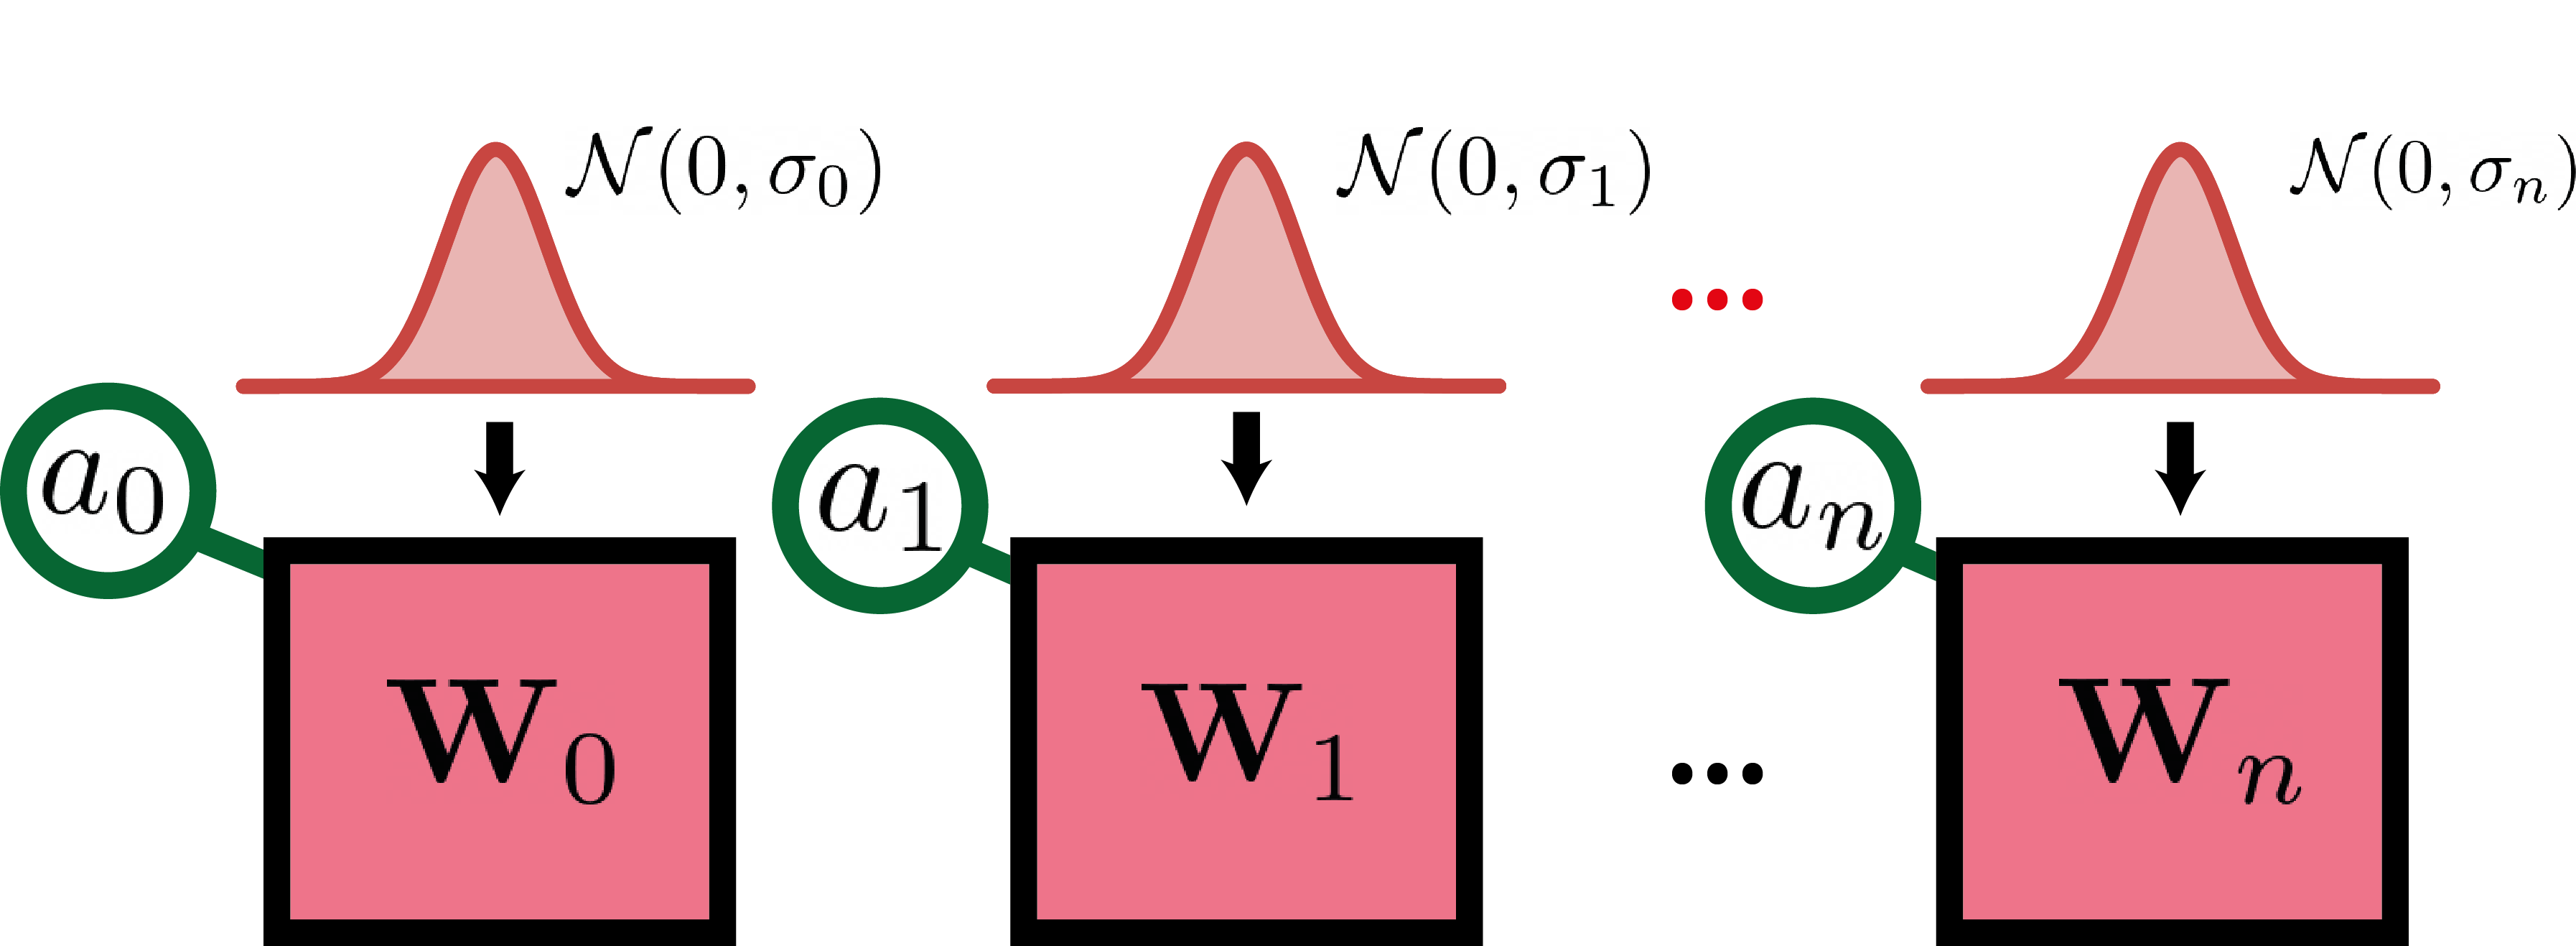
\includegraphics[width=\linewidth]{sections/1_adaptinit/imgs/adapt_init_2.png}
    \end{center}    
\end{frame}

\begin{frame}{Reparameterization Trick}

\textbf{Altering the value of \(a_i \in \mathbb{R}\)} is equivalent to \textbf{altering the initialization variance} of the corresponding layer, $\mathbf{W}_i \sim \mathcal{N}_{N_{i} \times N_{i-1}}\left(0, (\alpha_i \sigma_i)^2 \right)$.

    \begin{center}
        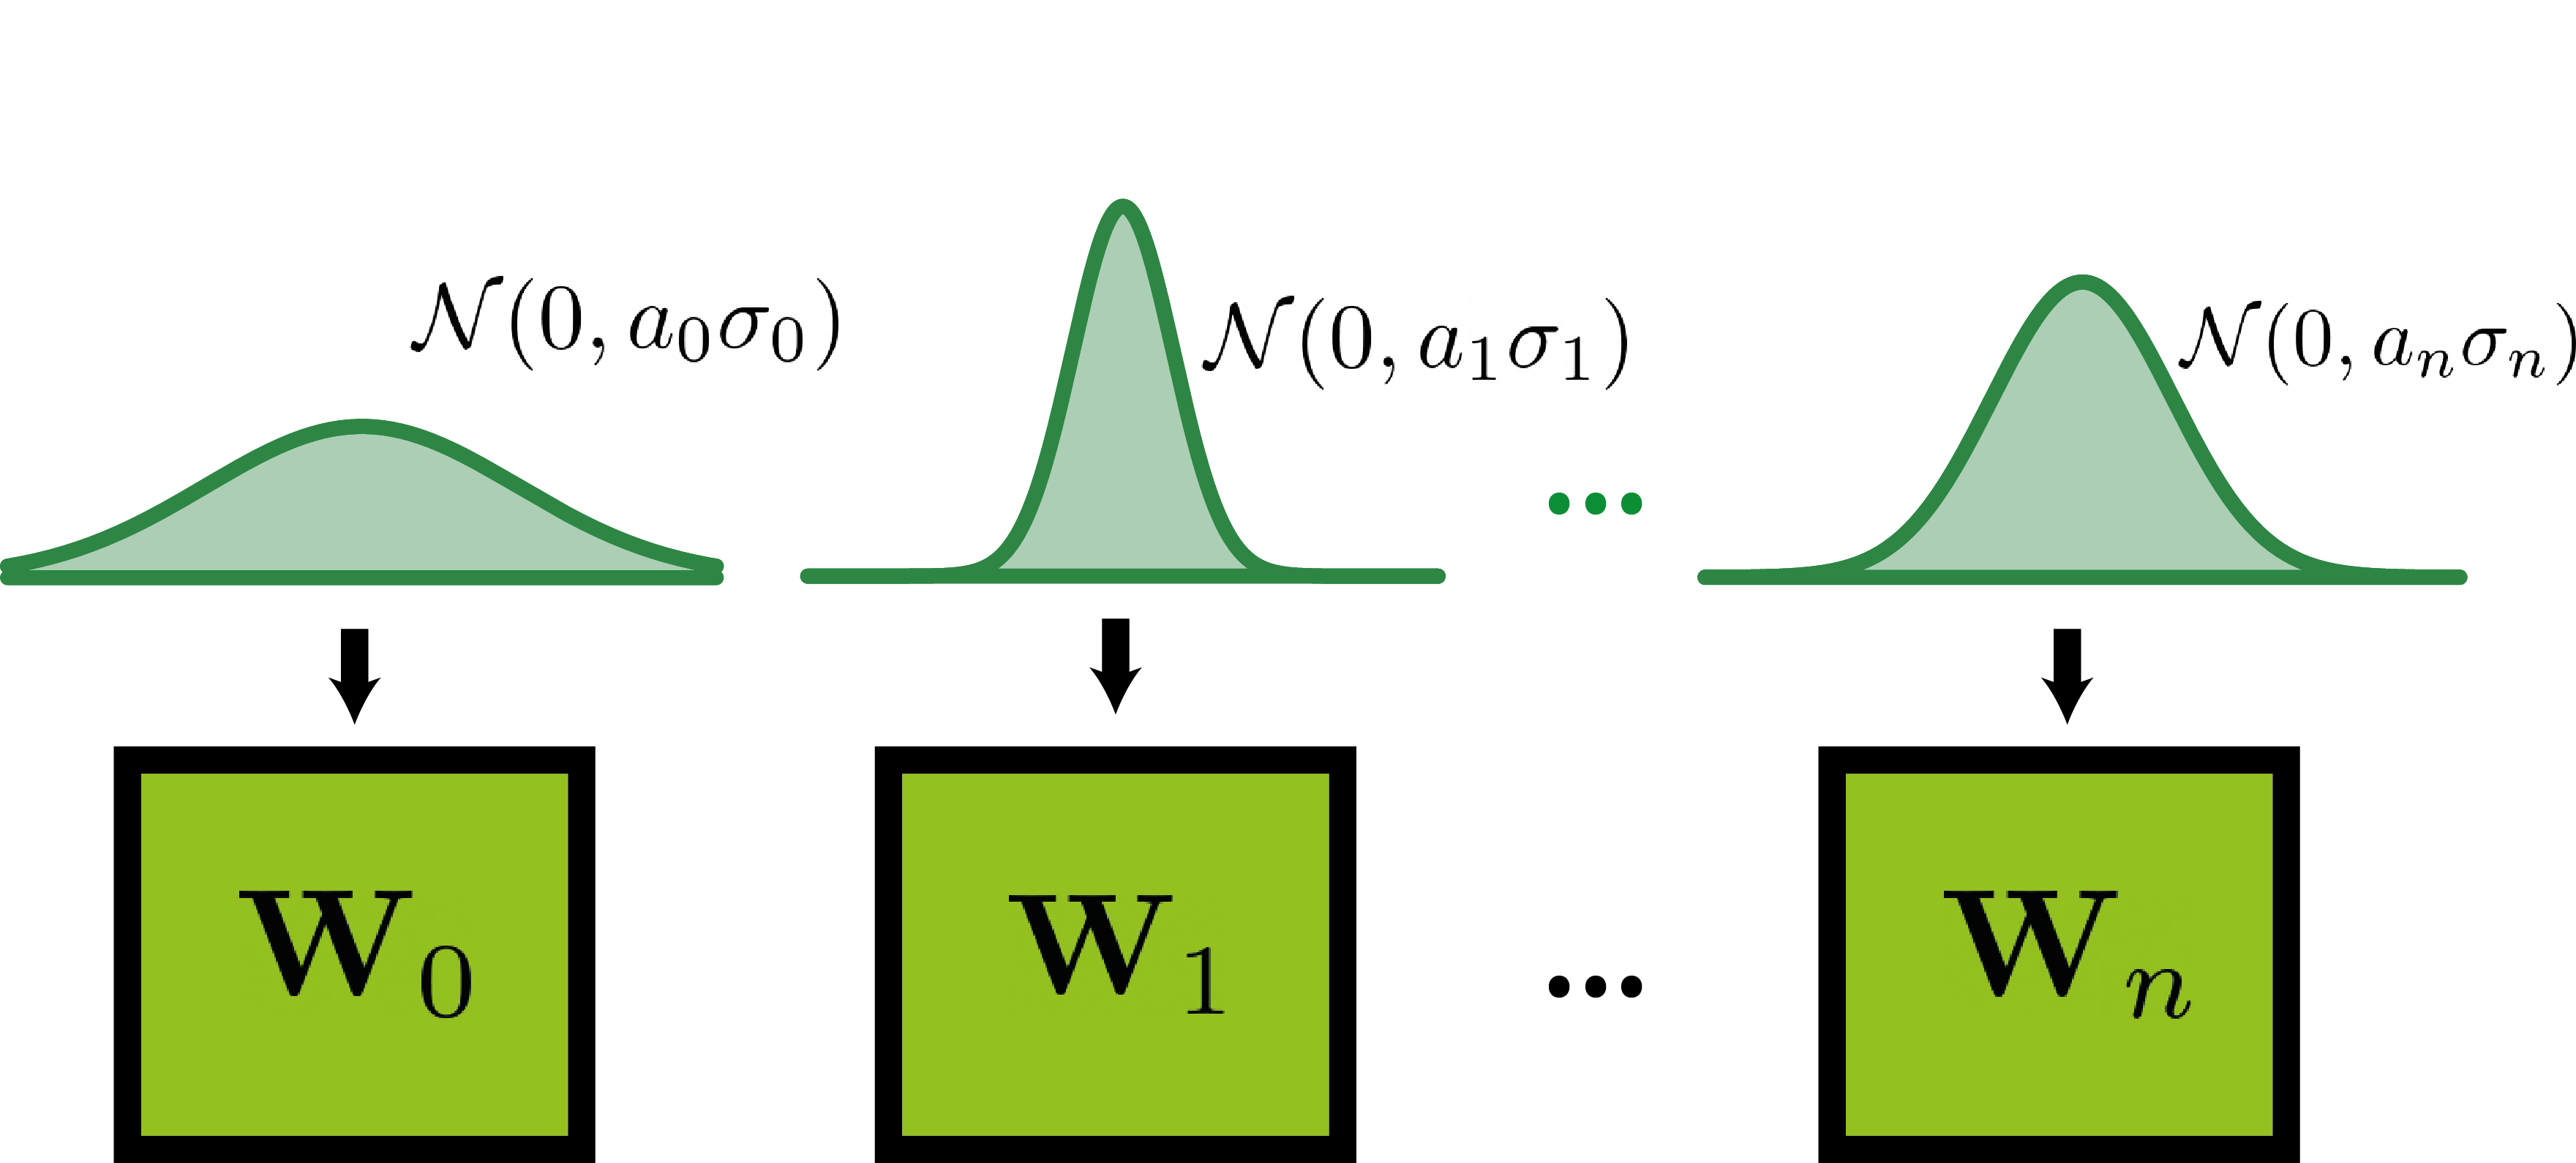
\includegraphics[width=\linewidth]{sections/1_adaptinit/imgs/adapt_init_3.png}    
    \end{center}
    
\end{frame}

% \begin{frame}
% 	Directly drawing values from a Gaussian distribution \(\mathcal{N}(\mu,
%   \sigma)\) that maximizes mutual information and initializing each layer's weights with them
%   would be the ideal scenario for an initialization scheme.
%   However, learning the parameters \(\mu \in \mathbb{R}\) and \(\sigma \in
%   \mathbb{R}\) directly is not 
%   possible, since the Gaussian distribution is not differentiable. What we propose
%   is to indirectly estimate them by fitting an estimator that we expect to work
%   best when the mutual information between the extracted representation and
%   the target variable is maximized. Moreover, estimating mutual information in
%   high-dimensional spaces is especially challenging and
%   inefficient.
% \end{frame}


% \begin{frame}
%   To this end, we can formulate an optimization problem based on the Data Processing Inequality to maximize the information for the \(k\)-th layer during the initialization:
% \begin{equation}
%     \begin{aligned}
%         \text{maximize } \quad &  I(Y_k, \hat{Y}), \text{ }  \forall k \in [0, M],\\
%         \text{s.t. } \quad &  \bm{W}_{k} \sim N(0,a_k\sigma^2), \\
%         & a_k > 0, \\
%     \end{aligned}
% \end{equation}
% {\scriptsize where \(M \in \mathbb{N}\) is the number of layers.}
% \end{frame}

\begin{frame}{Trainable Auxiliary Layer}
  % Since the Gaussian distribution is not differentiable and calculating the
  % information preserved for each layer is time consuming,
  % We propose to estimate the optimal variance for weight initialization
  % stochastically through an auxiliary classification task.

  The scaling  factor \(a_{i} \in \mathbb{R}\) is \textbf{progressively optimized} for
  each layer \textbf{through an auxiliary layer} 
    \begin{gather}
      \begin{split}
        \bm{y}_{k}^{class} & =  I_k^{adapt}(a_k, \bm{W}_k^{class}; \bm{x})\\
                          & = g^{class}(\bm{W}_k^{class}g_k(|a_k|\bm{W}_k
        f_{k-1}(\cdots(f_0(\bm{x})))) + \bm{b}_{k} \in \mathbb{R}^{N_c},
      \end{split}
    \end{gather}
{\scriptsize where \(\bm{x} \in \mathbb{R}^{N_0}\) is the input of the network and
\(\bm{W}_k^{class} \in \mathbb{R}^{N_c \times N_{k}}\).}

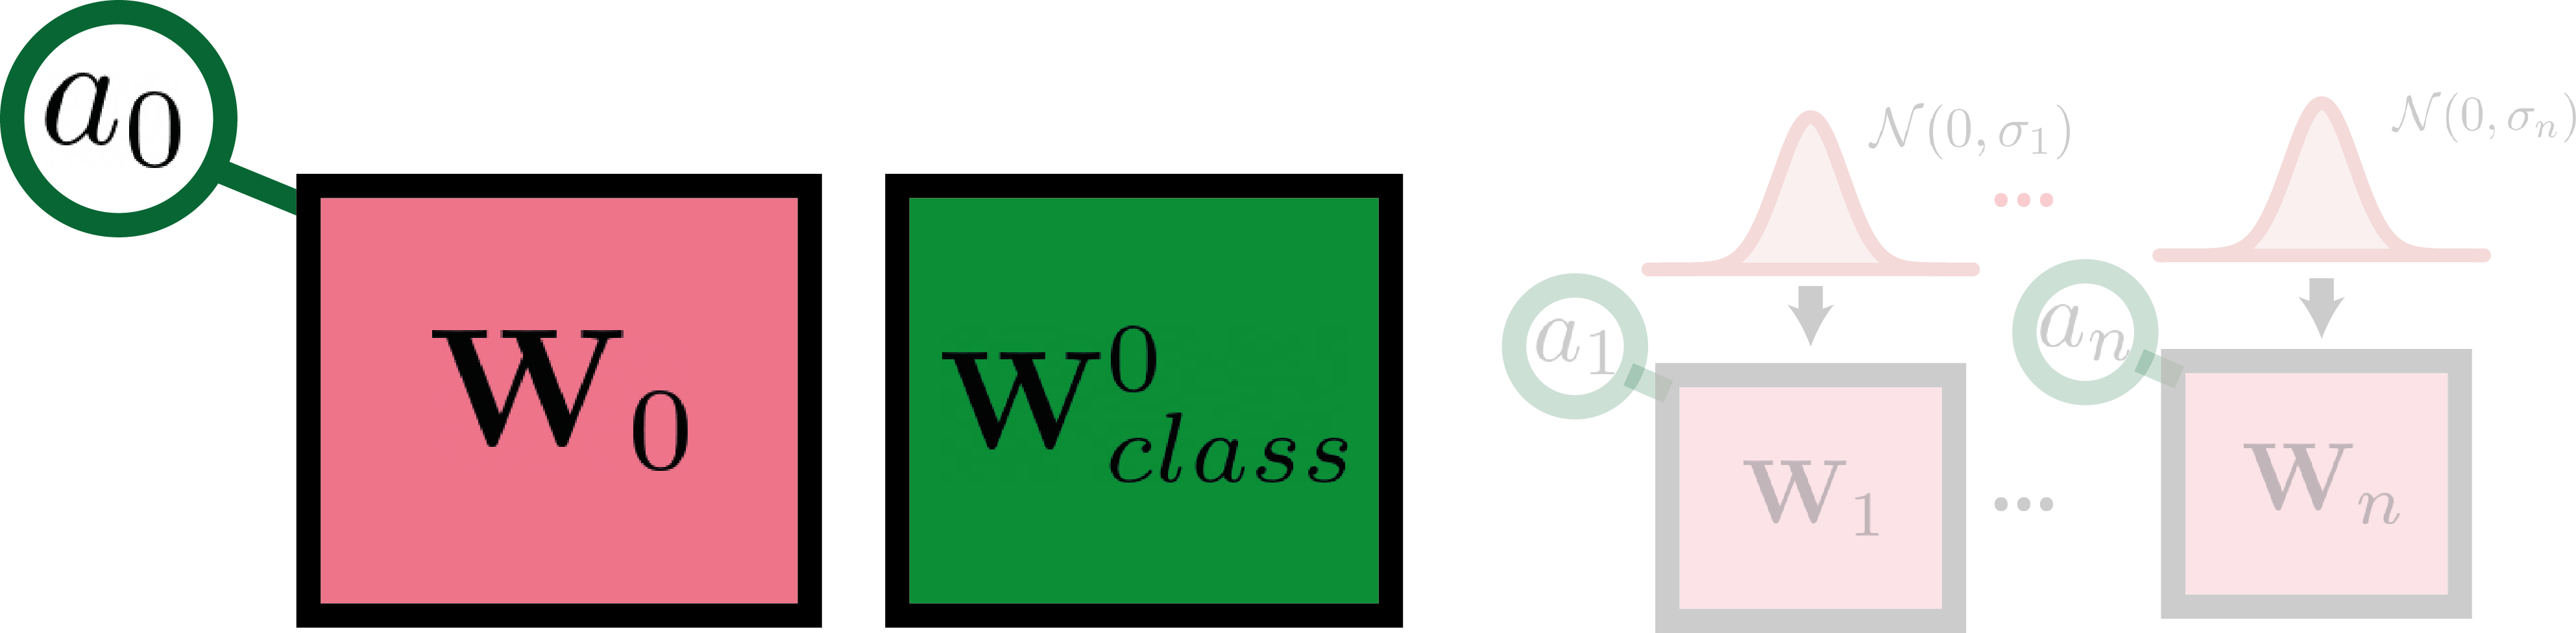
\includegraphics[width=\linewidth]{sections/1_adaptinit/imgs/adapt_init_4.png}
\end{frame}

% \begin{frame}{Regularization Term}
%   Since the proposed initialization targets to maximize the information
%   extracted from each layer, a regularization term is introduced to penalize
%   scaling factors that lead to saturated activation functions.
%   \begin{equation}
%     \tilde{J}(a_i, \bm{W}_i^{class}; \bm{x}, \bm{y}) = J(a_i, \bm{W}_i^{class}; \bm{x},
%     \bm{y}) + \gamma\Omega(\bm{z}_k) \in \mathbb{R},
%   \end{equation}
%   {\scriptsize where \(\gamma \in \mathbb{R}_+\) is the weighting factor for the penalty term.}

%   And \(\Omega(\cdot)\) is computed as:

% \end{frame}

% \begin{frame}{Optimization Process}
%   Finally, the scaling factor \(a_i \in \mathbb{R}_{+}\) and classification
%   weights \(\bm{W}_i^{class} \in \mathbb{R}^{M_{i} \times N_{c}}\) are optimized
%   using gradient descent: 
%   \begin{gather}
%     \Delta a_i = - \eta \frac{\partial \tilde{J}}{\partial a_i} - \gamma\frac{\partial
%     \Omega}{\partial a_i} \in \mathbb{R} \text{, } 
%   \Delta\bm{W}_i^{class} = - \eta \frac{\partial  \tilde{J}}{\partial\bm{W}_i^{class}} \in \mathbb{R}^{N_c \times N_k},
%   \end{gather}
%   {\scriptsize where \(\tilde{J}(\cdot)\) is the cost function used for network training,
%   \(\eta \in \mathbb{R}^{+}\) is the learning rate used, and \(c \in
%   \mathbb{R}^{+}\) is the weight of the relative contribution of the penalty
%   term, \(\Omega\).}

%   \begin{equation}
%     \Omega(\bm{z}_{k}) = \frac{\sum_{j=0}^{N_k}\max\{\lim_{x\to -\infty}g_k(x) - z_k, z_k - \lim_{x\to +\infty}g_k(x), 0\}}{N_{k-1} N_{k}} \in \mathbb{R},
%   \end{equation}
%   {\scriptsize where \(N_{i} \in \mathbb{N}\) and \(M_{i} \in \mathbb{N}\) is the fan-in and
%   fan-out respectively and \(\max\{\cdot\}\) denotes the maximum element in the
%   set.}
% \end{frame}

% \begin{frame}{Adaptive Initialization Pipeline}

% \vspace{15pt}

%     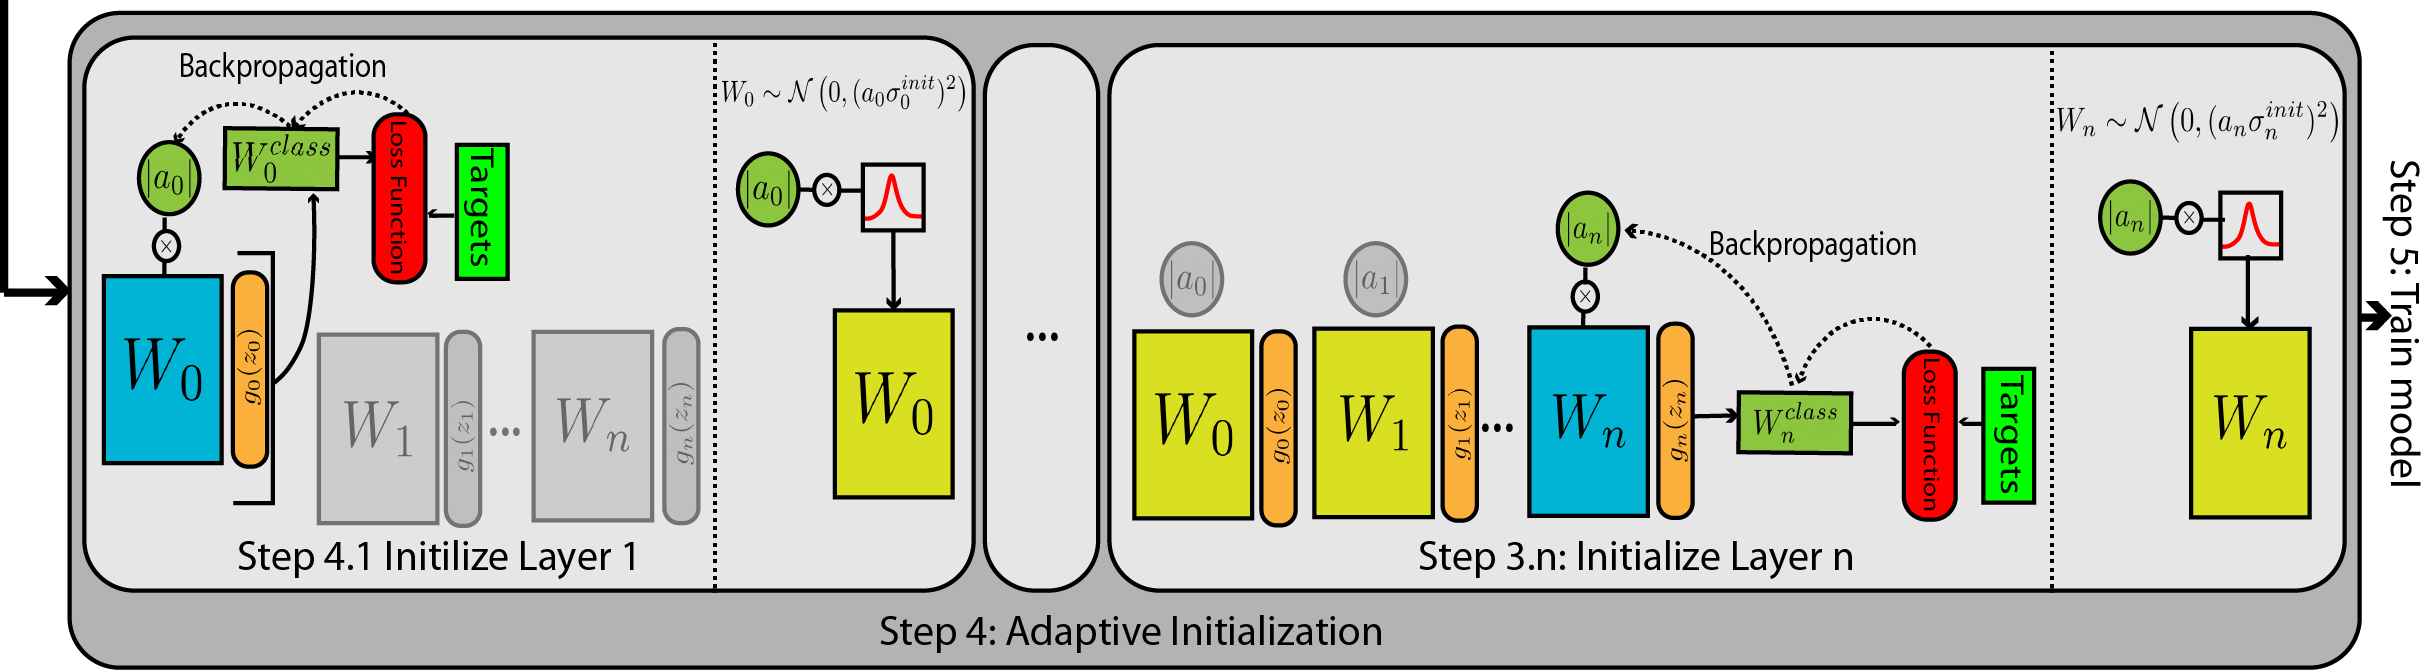
\includegraphics[width=\linewidth]{sections/1_adaptinit/imgs/adapt_init_5.png}


% \end{frame}


% \begin{frame}{Notes on proposed initialization}
% \begin{itemize}
%     \item The scale of the weights of the $i$-th layer are indirectly adapted
%       through $\alpha_i$ which is equivalent to initializing the layer with a
%       different variance.  
%     \item During the initialization process \textbf{none of the layers are
%         actually trained.} 
%     \item \textbf{The representations extracted from them are random
%         transformations/projections of the input data.} Such transformations
%       come with strong theoretical guarantees\footnote{Ali Rahimi et al. "Random
%         features for large-scale kernel machines." (NIPS'07)}. 
% \end{itemize}
% \end{frame}

\begin{frame}{Noise in Photonic Neuron}
\begin{center}
    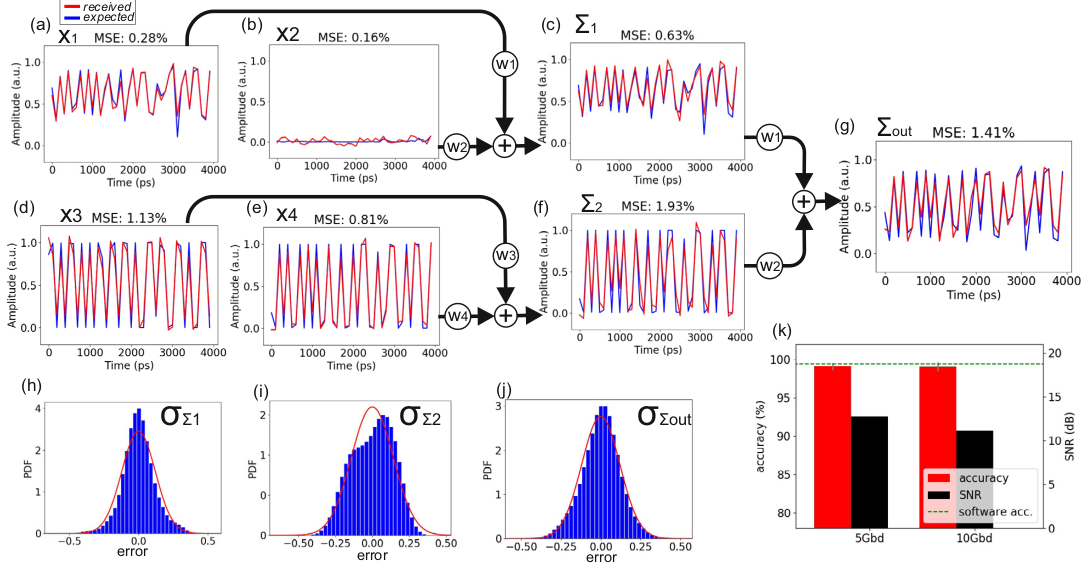
\includegraphics[width=0.9\linewidth]{sections/1_adaptinit/imgs/nature_no_noise.png}
\end{center} \vspace{-10pt}
  Different sources of noise can be \textbf{modeled} as a channel with an
   \textbf{Additive White Gaussian Noise (AWGN)}\footnote{\scriptsize Mourgias-Alexandris, G., Moralis-Pegios, M., Tsakyridis, A., Simos, S., Dabos, G., Totovic, A., Passalis, N., \textbf{Kirtas, M.}, Rutirawut, T., Gardes, F.Y. and Tefas, A., 2022.  \href{https://www.nature.com/articles/s41467-022-33259-z}{Noise-resilient and high-speed deep learning with coherent silicon photonics}. Nature communications, 13(1), p.5572} 
\end{frame}

\begin{frame}{Noise-aware Training}
  Exploiting the fact that \textbf{DL models are intrinsically resistant to noise},
  the proposed initialization treats noise as an intrinsic characteristic of the
  network.
  
    \begin{center}
        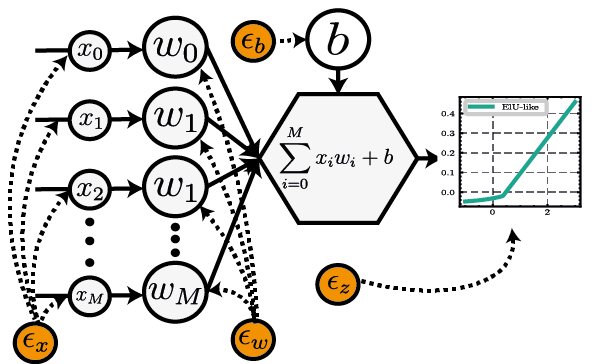
\includegraphics[width=0.6\linewidth]{sections/2_quant/imgs/quant_neuron.png}    
    \end{center}  
  \begin{equation*}
    z_{ij} =  {\sum_{j=1}^{N_k} \left( w_{ij} + \mathcal{N}(0, \sigma^2_w ) \right)}\left( x_{i-1,j} + \mathcal{N}(0, \sigma^2_x)\right) + \left(b_{i} + \mathcal{N}(0, \sigma^2_b)\right) \in \mathbb{R},
  \end{equation*}
  {\scriptsize where \(\sigma^2_x \in \mathbb{R}\), \(\sigma^2_w \in \mathbb{R}\) and  \(\sigma^2_b \in \mathbb{R}\) are the variances of the noise that
  affects the input, weighting, and bias mechanism, respectively.}
  
  % Thus, the basic noise sources and components of the DL system is
  % taken into account during training.
  % With the output of a noisy neuron modeled as:  
  
  %  And the final output of the neuron is modeled as:
  % \begin{equation}
  %   y_{ij} = g(u_{ij}) + \mathcal{N}(0, \sigma^2_g),
  % \end{equation}
  % {\scriptsize where \(\sigma^2_g\) is the variance of the noise induced by the activation
  % function.}
\end{frame}


% \begin{frame}{DL models - noise resistant}
%     Most of the existing works are \textbf{limited on evaluating the effect of
%       noise during the inference and after the network has already been
%       trained.} 
    
%     Overlooking the fact that DL models are \textbf{intrinsically resistant to
%       noise}, especially when they are first appropriately \textbf{trained to
%       withstand noisy signals.\footnote{N. Passalis, et al. , "Training Deep
%         Photonic Convolutional Neural Networks With Sinusoidal Activations,"
%         IEEE Transactions on Emerging Topics in Computational Intelligence,
%         (2019)}}\\ 
    
%     \vspace{0.5cm}
    
%     \textbf{\textcolor{mygreen}{A co-design approach can lead to significant
%         improvements.}} 
%       \end{frame}

\begin{frame}{Noise-aware Adaptive Initialization}
\begin{itemize}
    \item \textbf{After estimating the variance} for the first layer, the layer
      is appropriately re-initialized and \textbf{the weights
        $\mathbf{W}^{class}_i$ are discarded}.
    
    \item The initialization process \textbf{continues with the remaining layers.}

    \item \textbf{After all the layers have been initialized} using the proposed
       method, \textbf{the network is trained} in an end-to-end fashion. 
\end{itemize}

  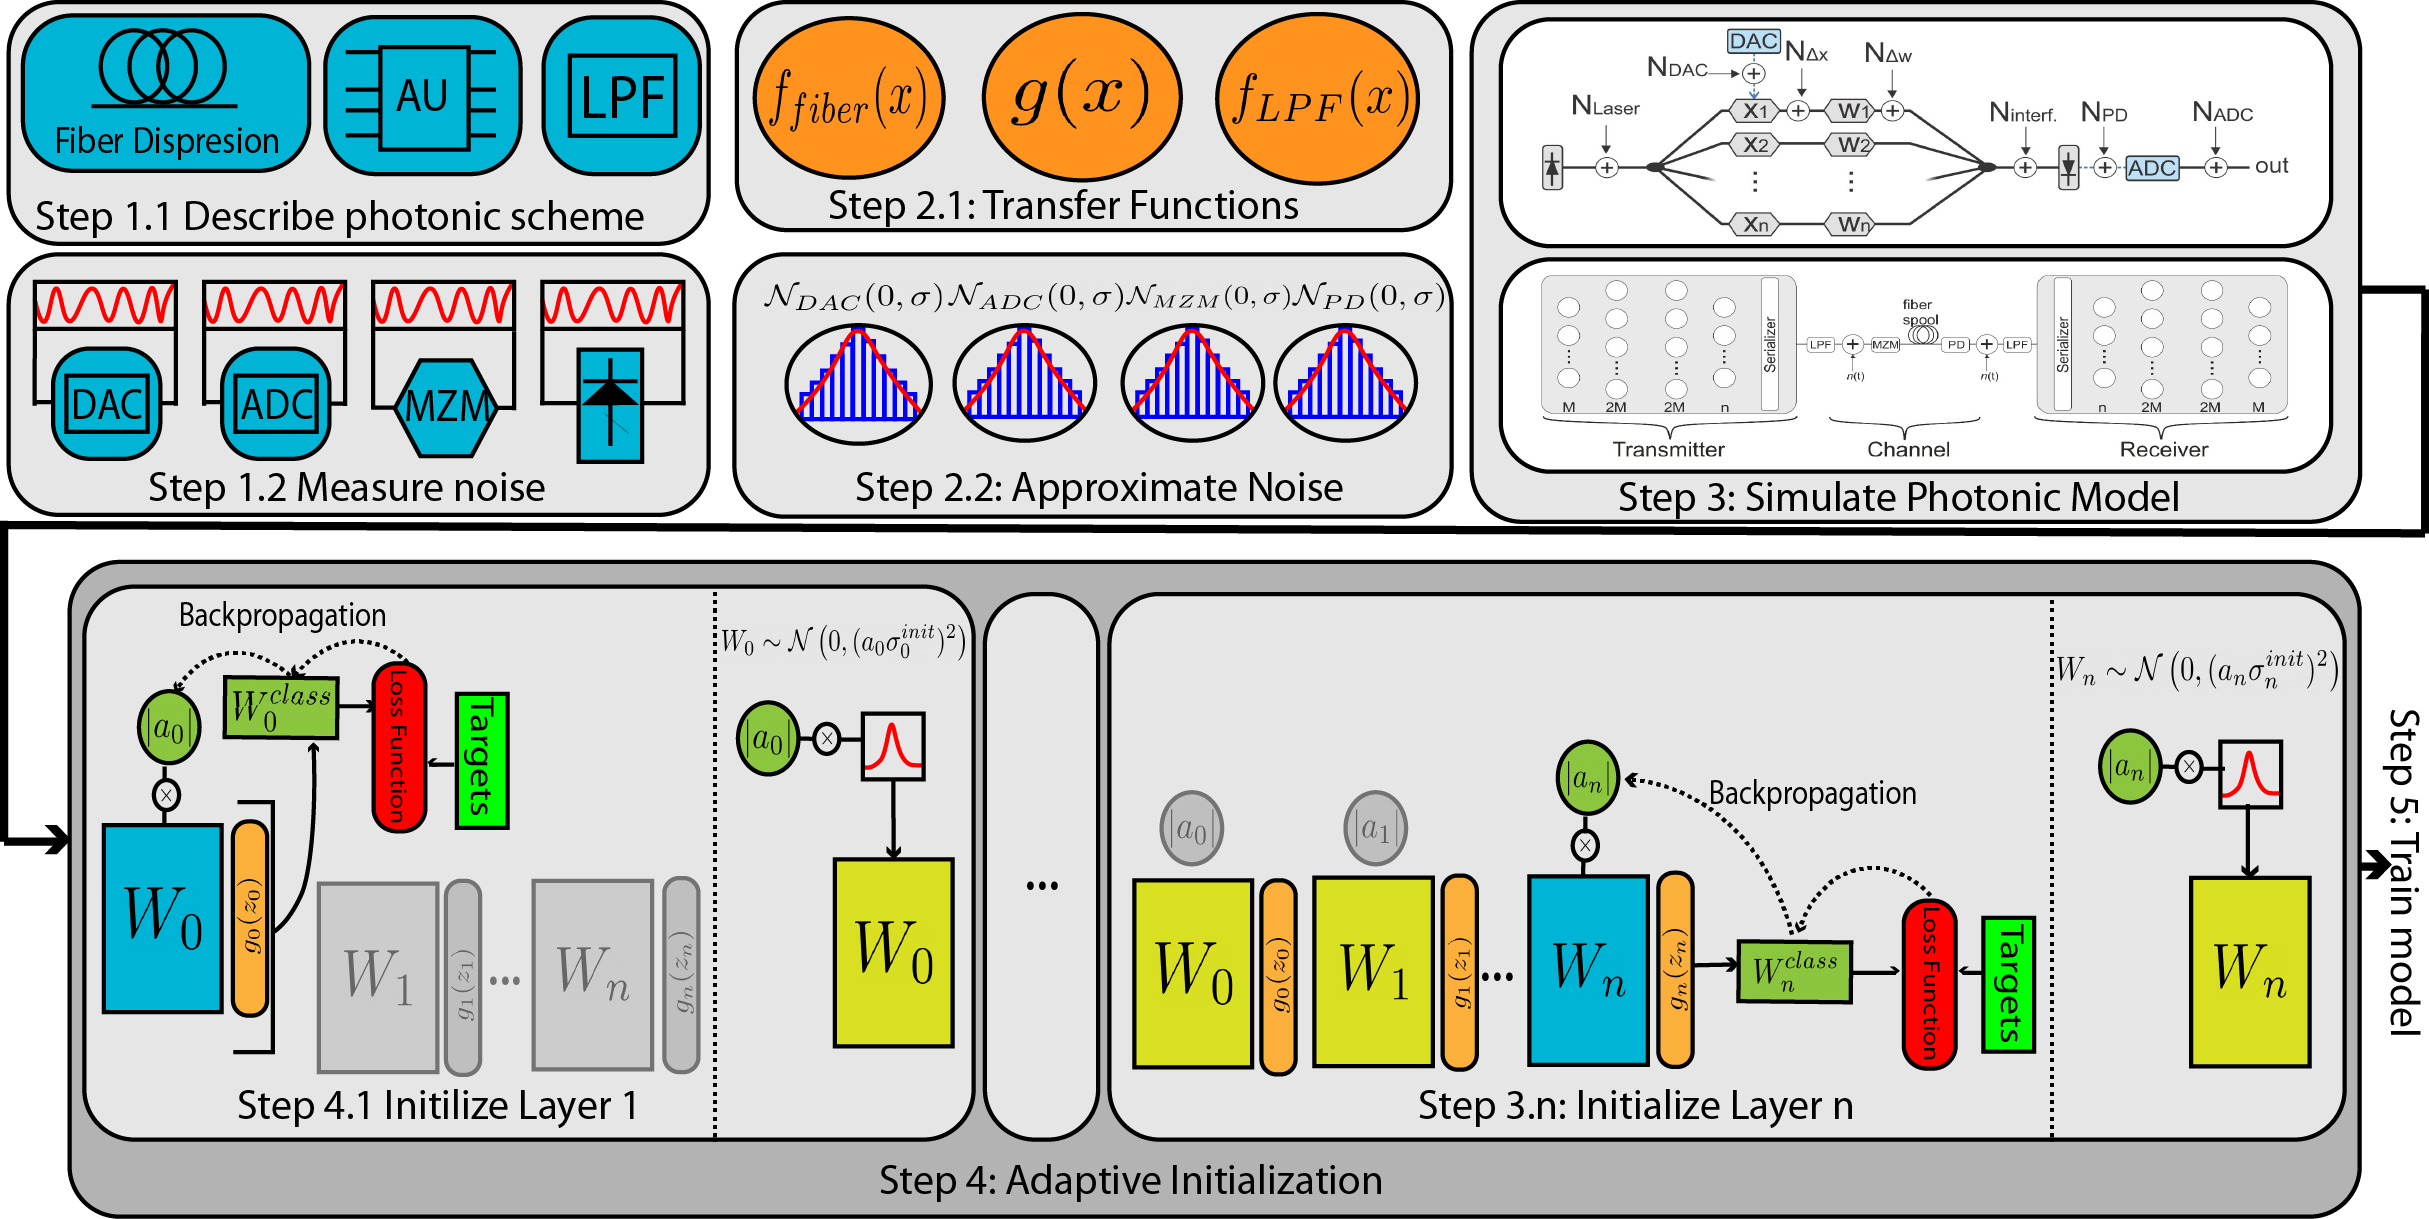
\includegraphics[width=\linewidth]{sections/1_adaptinit/imgs/Flow_diagram_new_latest.png}
\end{frame}

		
% \section{Experimental Evaluation}

% \section{Photonic Recurrent Networks}    
% \begin{frame}{FI-2010 Task}
% \begin{itemize}
%     \item For evaluating the proposed method, a challenging \textbf{large-scale high-frequency limit order book dataset (FI-2010)}\footnote{Paraskevi Nousi, et al., "Machine Learning for Forecasting Mid-Price Movements Using Limit Order Book Data" IEEE Access 7 (2019): 64722-64736} is employed. %~\cite{nousi2019machine}
%     \item The FI-2010 dataset contains more than \textbf{4 million limit orders collected from 5 Finnish companies.}
%     \item The forecasting task concerns the prediction of the \textbf{direction of the future mid-price movement} (up, down or stationary) after 10 time-steps.
% \end{itemize}
% \end{frame}

% \begin{frame}{Sigmoid-based recurrent photonic neurons}
%     The employed \textbf{recurrent photonic architecture} is composed of multiple recurrent photonic neurons. 
%     \begin{figure}  
%         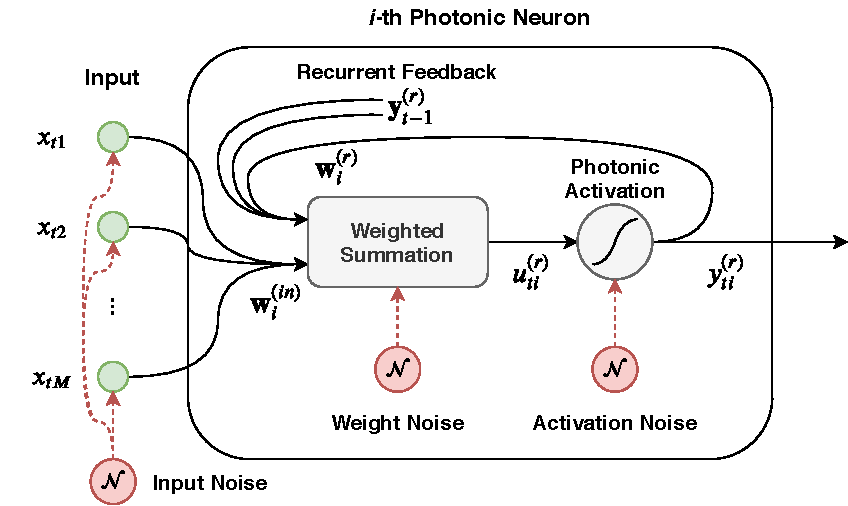
\includegraphics[scale=0.5]{sections/1_adaptinit/imgs/photonic_noisy.pdf}
%     \end{figure}
%      The final weighted output of the $i$-th recurrent neuron is then calculated as:
%     \begin{equation}
%     \label{eq:weighted-sum-rec}
%     u_{ti}^{(r)} = {\mathbf{w}_i^{(in)}}^T \mathbf{x}_{t} + {\mathbf{w}_i^{(r)}}^T \mathbf{y}^{(r)}_{t-1}.
%     \end{equation}
%     \begin{center}
%         \textit{  {\footnotesize Note that we omitted the bias term to simplify the employed notation.}}
%     \end{center}
% \end{frame}	

% \begin{frame}{Experimental Setup}
% \begin{itemize}
%     \item Photonic DL model for the conducted experiments is composed of:
%     \begin{itemize}
%         \item a recurrent photonic layer with 32 neuron
%         \item followed by two fully connected layers with 512 and 3 output respectively (same photonic architecture)
%     \end{itemize}
%     \item The length of the time series is 10
%     % \item Trained for 20 epochs with learning rate of \(\eta=10^{-4}\)
%     \item The scaling factor \(\alpha_i\):
%     \begin{itemize}
%         \item was estimated using 10 epochs with only 5 recurrent time steps
%         \item with learning rate 0.1 
%     \end{itemize}
%     % \item RMSprop optimization algorithm were used for both processes
%     \item The \(\kappa\) accuracy is used to measure the forecasting accuracy
% \end{itemize}

% \end{frame}



% \begin{frame}{FI2010 Dataset: Experimental Results}
%     \begin{table}
%     \label{table:eval}
%     \centering
%     \resizebox{0.85\linewidth}{!}{
%     \begin{tabular}{l|cccc}
%      $\sigma^2$  & Regular Training & Noisy Training & Adaptive Init. & Proposed  \\
%      \hline
%      \multicolumn{5}{c}{Weight Noise ($\sigma_w=\sigma, \sigma_{in}=\sigma_a=0$)}\\
%      \hline
%      .1 & 0.0807 & 0.1146 & 0.1498 & \textbf{0.1712} \\
%      .3 & 0.0486 & 0.1257 & 0.0809 & \textbf{0.1514} \\
%      .5 & 0.0138 & 0.1199 & 0.0096 & \textbf{0.1228} \\
%      \hline
%      \multicolumn{5}{c}{Activation Noise ($\sigma_a=\sigma, \sigma_{in}=\sigma_w=0$)}\\
%      \hline
%      .1 & 0.0884 & 0.1079 & 0.1693 & \textbf{0.1897} \\
%      .3 & 0.0681 & 0.1197 & 0.1410 & \textbf{0.1732} \\
%      .5 & 0.0267 & 0.1041 & 0.0674 & \textbf{0.1351} \\   
%     \hline
%      \multicolumn{5}{c}{Input noise ($\sigma_{in}=\sigma, \sigma_a=\sigma_w=0$)}\\
%      \hline
%     .1 & 0.0923 & 0.1102 & 0.1324 & \textbf{0.1626} \\
%     .3 & 0.0635 & 0.1128 & 0.0975 & \textbf{0.1632} \\
%     .5 & 0.0179 & 0.1003 & 0.0381 & \textbf{0.1068} \\
%     \hline
%       \multicolumn{5}{c}{Weight/Activation/Input Noise  ($\sigma_{in}=\sigma_a=\sigma_w=\sigma$)}\\
%      \midrule
%      .1 & 0.0627 & 0.1195 & 0.1351 & \textbf{0.1566} \\
%      .3 & 0.0274 & 0.1085 & 0.0552 & \textbf{0.1253} \\
%      .5 & 0.0058 & 0.0917 & 0.0078 & \textbf{0.1000} \\
%      \hline
%      \multicolumn{5}{c}{No noise  + Adaptive Initialization: 0.1738}\\
%     \end{tabular}}
%     \vspace{-1em}
%     \end{table}
% \end{frame}	

% \begin{frame}{Image Classification: Experimental Results}
%   \begin{table}
%   \centering
%   \resizebox{.83\linewidth}{!}{
%   \begin{tabular}{l|c|c|c|c||c|c|c|c}
%     & \multicolumn{4}{c||}{FashionMNIST}  &  \multicolumn{4}{c}{CIFAR10} \\
%     \midrule
%     & \multicolumn{8}{c}{\thead{Noise Level}} \\
%     \midrule
%     Initialization & 0.0 & 0.05 & 0.1 & 0.2 & 0.0 & 0.05 & 0.1 & 0.2 \\
%     \midrule
%     & \multicolumn{8}{c}{Photonic Sigmoid}\\
%     \midrule
%     Xavier & $ 17.88 $ &	$ 23.31 $  & $ 29.36  $ &  $ 89.57 $ & $ 90.0 $ & $ 89.77 $  & $ 89.9  $ &  $ 90.33 $\\
%     \textbf{+ Proposed}  &\bm{$ 8.63 $} &  \bm{$ 12.4 $} & \bm{$ 19.21 $} &  \bm{$ 25.16 $} &\bm{$ 20.52 $} &  \bm{$ 29.4 $} & \bm{$ 37.33 $} &  \bm{$ 56.01 $}\\
%     \midrule
%     He  & $ 19.17 $ & $ 23.45 $ & $ 28.29 $ & $ 29.23 $  & $ 74.17 $ & $ 89.54 $ & $ 90.14 $ & $ 90.0 $  \\
%     \textbf{+ Proposed}   & \bm{$ 9.06 $} & \bm{$ 12.81 $} & \bm{$ 21.53 $} & \bm{$ 26.73 $} & \bm{$ 25.18 $} & \bm{$ 28.23 $} & \bm{$ 39.94 $} & \bm{$ 89.82 $}\\
%     \midrule
%     & \multicolumn{8}{c}{Photonic Sinusoidal}\\
%     \midrule
%     Xavier & $ 8.04 $  & $ 9.4 $  &  $ 11.85 $ & $ 28.83 $ & $ 18.62 $  & $ 21.06 $  &  $ 28.2 $ & $ 74.23 $\\
%     + Proposed & \bm{$ 7.65 $} &  \bm{$ 8.82 $} & \bm{$ 10.48 $} &  \bm{$ 16.75 $} &\bm{$ 16.36 $} &  \bm{$ 19.47 $} & \bm{$ 24.97 $} &  \bm{$ 41.55 $}\\
%     \midrule
%     % \cdashline{2-7}
%     He  &  $  9.16 $ & $ 10.22 $ & $ 14.51 $ & $ 24.38 $ &  $ 52.28 $ & $ 43.92 $ & $ 56.3 $ & $ 90.3 $ \\
%     \textbf{+ Proposed}  & \bm{$ 8.62 $} & \bm{ $ 9.54 $} & \bm{$ 12.0 $} & \bm{$ 16.03 $} & \bm{$ 21.67 $} & \bm{ $ 21.74 $} & \bm{$ 28.47 $} & \bm{$ 48.85 $}\\
%     \midrule
%     & \multicolumn{8}{c}{Sigmoid}\\
%     \midrule
%     Xavier & $ 90.0 $  & $58.46$  & $89.65$ &  $90.08$ & $ 90.0 $  & $ 89.97 $  & $ 89.53 $ &  $ 90.03 $ \\
%     \textbf{+ Proposed}  &\bm{$ 8.74 $} &  \bm{$ 9.11 $} & \bm{$ 11.14 $} &  \bm{$ 15.29 $} &\bm{$ 20.54 $} &  \bm{$ 25.93 $} & \bm{$ 25.75 $} &  \bm{$ 35.64 $}\\ 
%     \midrule
%     He   & $ 13.67  $ & $ 14.09 $ & $ 15.42 $ &  $ 18.66 $ & $ 90.0  $ & $ 90.63 $ & $ 89.98 $ &  $ 90.43 $\\
%     \textbf{+ Proposed}   & \bm{$ 8.81 $} & \bm{$ 10.26 $} & \bm{$ 12.37 $} & \bm{$ 16.18 $} & \bm{$ 23.81 $} & \bm{$ 25.33 $} & \bm{$ 32.21 $} & \bm{$ 42.45 $}\\
%     \midrule
%     \bottomrule
%   \end{tabular}}
% \end{table}
% \end{frame}

% \section{Optical Fiber Communication}

% \begin{frame}{Experimental Setup}
%     \begin{itemize}
%         \item  Proposed method is employed on an intensity modulation/direct detection(IM/DD) system which is \textbf{trained in an end-to-end fashion as a single feed-forward ANN}
%         \item The system is composed of a \textbf{neural transmitter, a channel and a neural receiver.} 
%         \item The channel introduces a \textbf{non-linear transfer function with noise} due to the fiber dispersion.
%         \item \textbf{Goal} is to obtain the signal in receiver with the \textbf{minimum Bit Error Rate} (BER) after transmitting it through the noisy channel.
%     \end{itemize}
% \end{frame}

% \begin{frame}{Experimental Setup}
%     \begin{figure}
%         \centering
%         % \includegraphics[scale=0.3]{images/fiber_link.jpg}
%     \end{figure}
    
%     \begin{itemize}
%         \item the input of the transmitter model, which is a 6-bit symbol, is \textbf{encoded in a one-hot-vector of size 64}.
%         \item transmitter is a \textbf{fully connected 3-layer feed-forward ANN}.
%         \item receiver gets the deserialized output of the channel as an input of \(n\) symbols.
%         \textbf{Receiver} consists of \textbf{2-hidden layers and an output layer} with softmax activation function.
%         \item both a photonic \textbf{sigmoid-based} architecture, as well as a \textbf{sinusoidal-based} architecture are employed
%     \end{itemize}
% \end{frame}


\begin{frame}{Optical Fiber Communication: Setup}
\begin{center}
    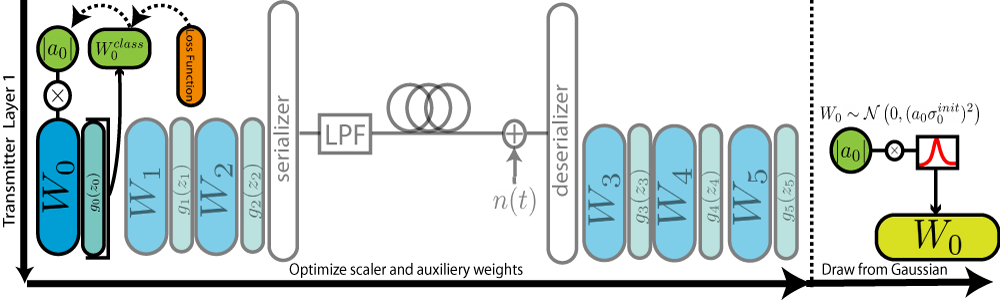
\includegraphics[width=\linewidth]{sections/1_adaptinit/imgs/pt1_flow.png}
    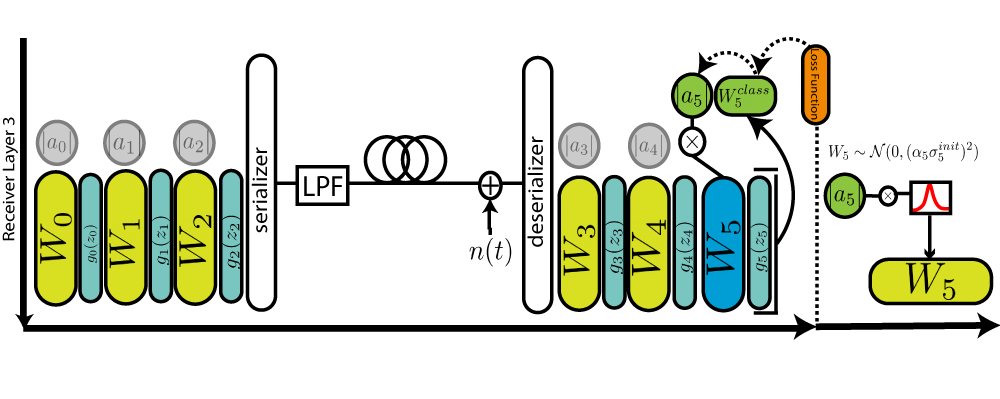
\includegraphics[width=\linewidth]{sections/1_adaptinit/imgs/pt2_flow.png}
\end{center}
\end{frame}


% \begin{frame}{Optical Fiber Communication:  Initialize Receiver}
%     \begin{figure}
%         \centering
%         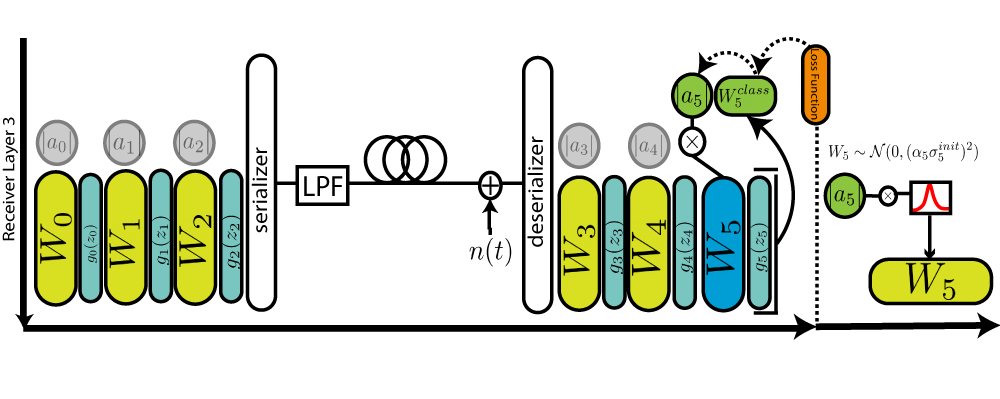
\includegraphics[width=\linewidth]{sections/1_adaptinit/imgs/pt2_flow.png}
%         \caption{Initialize third layer of receiver}
%         \label{fig:my_label}
%     \end{figure}
% \end{frame}


\begin{frame}{Optical Fiber Communication: Experimental Results}
\begin{table}
  \centering
  \resizebox{.83\linewidth}{!}{
  \begin{tabular}{p{0.5cm}|cc|cc}
  \(L\) & Xavier & + Proposed & He & + Proposed\\
     \hline
   & \multicolumn{4}{c}{Sigmoid} \\
    \hline
  30 & $ 7.38\times 10^{-3} $ & \bm{$ 5.65\times 10^{-5} $} & $ 9.90\times 10^{-4} $  & \bm{$ 8.20\times 10^{-5} $}\\
  40 & $ 5.15\times 10^{-3} $ & \bm{$ 3.41\times 10^{-3} $} & $ 3.26\times 10^{-3} $ & \bm{$ 3.68\times 10^{-4} $}\\
  50 & $ 1.11\times 10^{-2} $ & \bm{$ 4.79\times 10^{-3} $} & $ 5.30\times 10^{-3} $  & \bm{$ 1.39\times 10^{-3} $}\\
  60 & $ 7.38\times 10^{-3} $ & \bm{$ 3.06\times 10^{-3} $} & $ 7.66\times 10^{-3} $ & \bm{$ 2.77\times 10^{-3} $}\\
  70 & $ 6.94\times 10^{-3} $ & \bm{$ 5.85\times 10^{-3} $} & $ 6.76\times 10^{-3} $ & \bm{$ 5.42\times 10^{-3} $}\\
   \hline
   & \multicolumn{4}{c}{Photonic Sigmoid} \\
    \hline
  30 & $ 2.31\times 10^{-4} $ & \bm{$ 3.14\times 10^{-5} $} & $ 1.23\times 10^{-3} $ & \bm{$ 6.86\times 10^{-5} $}\\ 
  40 & $ 1.63\times 10^{-3} $ & \bm{$ 2.21\times 10^{-4} $} & $ 3.04\times 10^{-3} $ & \bm{$ 2.74\times 10^{-4} $}\\
  50 & $ 2.93\times 10^{-3} $ & \bm{$ 1.31\times 10^{-3} $} & $ 5.06\times 10^{-3} $ & \bm{$ 1.70\times 10^{-3} $}\\
  60 & $ 6.49\times 10^{-3} $ & \bm{$ 1.97\times 10^{-3} $} & $ 8.01\times 10^{-3} $ & \bm{$ 4.08\times 10^{-3} $}\\
  70 & $ 6.38\times 10^{-3} $ & \bm{$ 2.34\times 10^{-3} $} & $ 8.27\times 10^{-3} $ & \bm{$ 5.03\times 10^{-3} $}\\
  \hline
  & \multicolumn{4}{c}{Photonic Sinusoidal}\\
  \hline
    30 & $ 1.53\times 10^{-5} $ & \bm{$ 1.17\times 10^{-5} $} & $ 2.91\times 10^{-5} $ & \bm{$ 1.02\times 10^{-5} $}\\
  40 & $ 6.30\times 10^{-5} $ & \bm{$ 6.28\times 10^{-5} $} & $ 1.20\times 10^{-4} $ & \bm{$ 1.18\times 10^{-4} $}\\
  50 & $ 3.70\times 10^{-4} $ & \bm{$ 3.15\times 10^{-4} $} & $ 9.65\times 10^{-4} $ & \bm{$ 4.32\times 10^{-4} $}\\
  60 & $ 1.27\times 10^{-3} $ & \bm{$ 9.18\times 10^{-4} $} & $ 1.95\times 10^{-3} $ & \bm{$ 1.80\times 10^{-3} $}\\
  70 & $ 2.11\times 10^{-3} $ & \bm{$ 1.49\times 10^{-3} $} & $ 3.46\times 10^{-3} $ & \bm{$ 2.27\times 10^{-3} $}\\
    \hline
 \end{tabular}}
 \label{tab:eval-loss}
\end{table}
\end{frame}

\begin{frame}{Publications}
\begin{itemize}
    \item Main Journal Publications
    \begin{itemize}
        \item {\scriptsize \textbf{Kirtas, M.}, Passalis, N., Mourgias-Alexandris, G., Dabos, G.,
      Pleros, N. and Tefas, A., 2022. \href{https://ieeexplore.ieee.org/document/9815870}{Robust architecture-agnostic and noise resilient training of photonic deep learning models.} IEEE Transactions on Emerging Topics in Computational Intelligence.} 
    \end{itemize}
    \item Main Conference Publications 
        \begin{itemize}
        \item {\scriptsize \textbf{Kirtas, M.}, Passalis, N., Mourgias-Alexandris, G., Dabos, G., Pleros, N. and Tefas, A., 2022, August. \href{https://ieeexplore.ieee.org/abstract/document/9909781}{Learning photonic neural network initialization for noise-aware end-to-end fiber transmission.} In 2022 30th European signal processing conference (EUSIPCO)}
    \end{itemize}
    % \item Relevant Journal Publications
    %     \begin{itemize}
    %     \item 
    % \end{itemize}
    % \item Relevant Conference Publications
    %     \begin{itemize}
    %     \item {\scriptsize Passalis, N., \textbf{Kirtas, M.}, Mourgias-Alexandris, G., Dabos, G.,
    %   Pleros, N. and Tefas, A., 2021, January.\href{https://ieeexplore.ieee.org/abstract/document/9287649}{Training noise-resilient recurrent photonic networks for financial time series analysis.} In 2020 28th European Signal Processing Conference (EUSIPCO)}

    
\end{itemize}
\end{frame}



%   \begin{table}
%   \caption{FashionMNIST - Classification Error (\%)  for Different Activation Functions and Noise Levels}
%   \centering
%   \begin{tabular}{l|c|c|c|c||c|c|c|c}
%     & \multicolumn{4}{c||}{FashionMNIST}  &  \multicolumn{4}{c}{CIFAR10} \\
%     \midrule
%     & \multicolumn{8}{c}{\thead{Noise Level}} \\
%     \midrule
%     Initialization & 0.0 & 0.05 & 0.1 & 0.2 & 0.0 & 0.05 & 0.1 & 0.2 \\
%     \midrule
%     & \multicolumn{8}{c}{Sigmoid}\\
%     \midrule
%     Xavier & $ 90.0 $  & $ 89.97 $  & $ 89.53 $ &  $ 90.03 $ \\
%     &\bm{$ 20.54 $} &  \bm{$ 25.93 $} & \bm{$ 25.75 $} &  \bm{$ 35.64 $}\\ 
%     \midrule
%     He   & $ 90.0  $ & $ 90.63 $ & $ 89.98 $ &  $ 90.43 $\\
%     \textbf{+ Proposed}   & \bm{$ 23.81 $} & \bm{$ 25.33 $} & \bm{$ 32.21 $} & \bm{$ 42.45 $}\\
%     \midrule
%     & \multicolumn{8}{c}{Photonic Sigmoid}\\
%     \midrule
%     Xavier  & $ 90.0 $ & $ 89.77 $  & $ 89.9  $ &  $ 90.33 $\\
%     \textbf{+ Proposed}  &\bm{$ 20.52 $} &  \bm{$ 29.4 $} & \bm{$ 37.33 $} &  \bm{$ 56.01 $}\\
%     He  & $ 74.17 $ & $ 89.54 $ & $ 90.14 $ & $ 90.0 $  \\
%     \textbf{+ Proposed}   & \bm{$ 25.18 $} & \bm{$ 28.23 $} & \bm{$ 39.94 $} & \bm{$ 89.82 $}\\
%     \midrule
%     & \multicolumn{8}{c}{Photonic Sinusoidal}\\
%     \midrule
%     Xavier & $ 18.62 $  & $ 21.06 $  &  $ 28.2 $ & $ 74.23 $\\
%     + Proposed &\bm{$ 16.36 $} &  \bm{$ 19.47 $} & \bm{$ 24.97 $} &  \bm{$ 41.55 $}\\
%     \midrule
%     % \cdashline{2-7}
%     He  & $ 52.28 $ & $ 43.92 $ & $ 56.3 $ & $ 90.3 $ \\
%     \textbf{+ Proposed}  & \bm{$ 21.67 $} & \bm{ $ 21.74 $} & \bm{$ 28.47 $} & \bm{$ 48.85 $}\\
%     \bottomrule
%   \end{tabular}
%   \label{tab:1_fashion_mnist}
% \end{table}



% \begin{frame}
% 	To this end, we propose an auxiliary
%   task based on the expectations that mutual information increases when the
%   loss between the extracted representation and the target variable is minimized.
%   In this way, fitting an auxiliary classification (or regression) layer can be
%   used as a proxy approximator. The motivation behind the proposed approach is
%   that if \(I(\hat{X}_i; Y)\) is maintained, then a simple linear classifier would
%   be able to extract some useful information about \(Y\). Therefore, instead of
%   directly learning the distribution parameters to maximize \(I(\hat{X}_i; Y)\),
%   we can efficiently optimize the parameters to maximize the information that can
%   be extracted using a linear classifier. Apart from using an efficient proxy for
%   optimization, a re-parameterization approach is also employed, which allows us
%   to draw from the fixed distribution \(\mathcal{N}(0, 1)\) which in turn is
%   appropriately scaled and translated using trainable parameters by intercepting a
%   classification-based proxy instead of quantitatively measuring mutual
%   information. This allows for effectively learning the initialization variance
%   using regular back-propagation, since instead of back-propagating the gradients
%   through the (non-differential) Gaussian distribution, we employ a differentiable
%   scaling scheme over it.
% \end{frame}
